% Created 2022-03-18 Fri 08:36
% Intended LaTeX compiler: pdflatex
\documentclass[11pt]{article}
\usepackage[utf8]{inputenc}
\usepackage[T1]{fontenc}
\usepackage{graphicx}
\usepackage{longtable}
\usepackage{wrapfig}
\usepackage{rotating}
\usepackage[normalem]{ulem}
\usepackage{amsmath}
\usepackage{amssymb}
\usepackage{capt-of}
\usepackage{hyperref}
\usepackage{color}
\usepackage{listings}
\usepackage{placeins}
\author{Nathan Vercaemert}
\date{2022-03-16}
\title{Sorts\\\medskip
\large CSC 505 Spring 2022 (001)}
\hypersetup{
 pdfauthor={Nathan Vercaemert},
 pdftitle={Sorts},
 pdfkeywords={},
 pdfsubject={},
 pdfcreator={Emacs 27.2 (Org mode 9.5.1)}, 
 pdflang={English}}
\begin{document}

\maketitle
\tableofcontents

\section{Insertion Sort}
\label{sec:orgff32f52}
MIT OCW Introduction to Algorithms 6.046J/18.401J LECTURE 1
\begin{center}
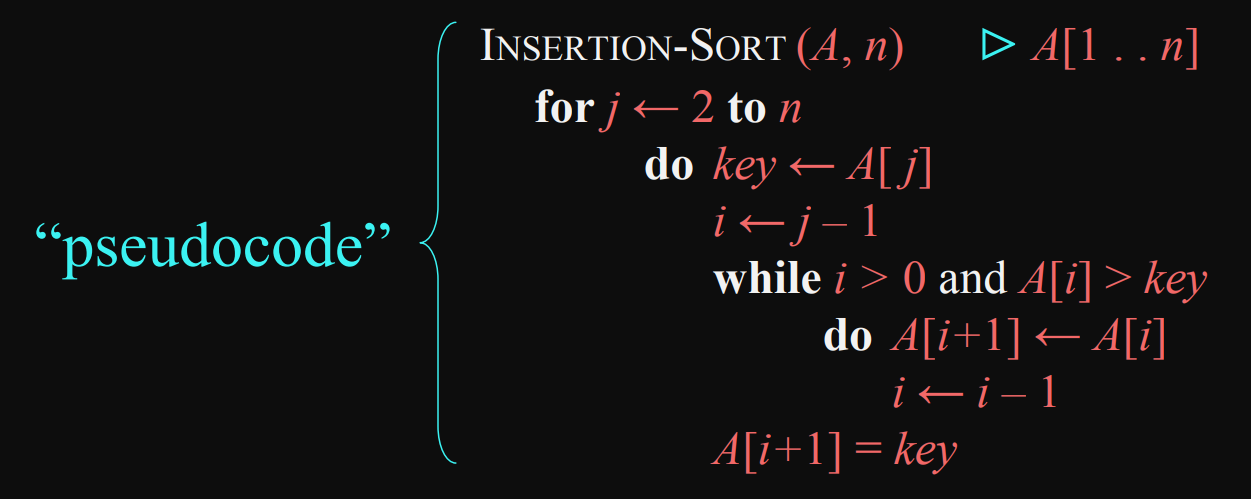
\includegraphics[width=.9\linewidth]{./Screenshot 2022-03-16 095958.png}
\end{center}
\subsection{Stack Overflow}
\label{sec:org857b812}
\url{https://stackoverflow.com/questions/12755568/how-does-python-insertion-sort-work}
Title: How does Python insertion sort work?
\begin{center}
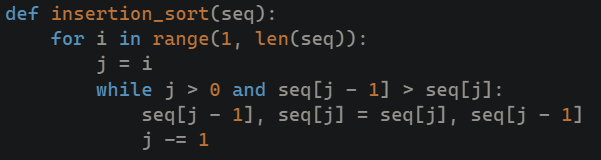
\includegraphics[width=.9\linewidth]{./Screenshot 2022-03-16 100657.png}
\end{center}
\subsection{Changes}
\label{sec:org7a7682b}
\begin{itemize}
\item Variable names were changed for consistency with mergeSort.
\item Operator was switched to "less than" for consistency.
\end{itemize}
\subsubsection{Note}
\label{sec:orgfb6e647}
Psuedocode does not exactly match implementation, but close inspection will reveal that the execution matches psuedocode.
\section{Merge Sort}
\label{sec:org4bc3642}
MIT OCW SEARCHING AND SORTING ALGORITHMS 6.0001 LECTURE 12
\begin{center}
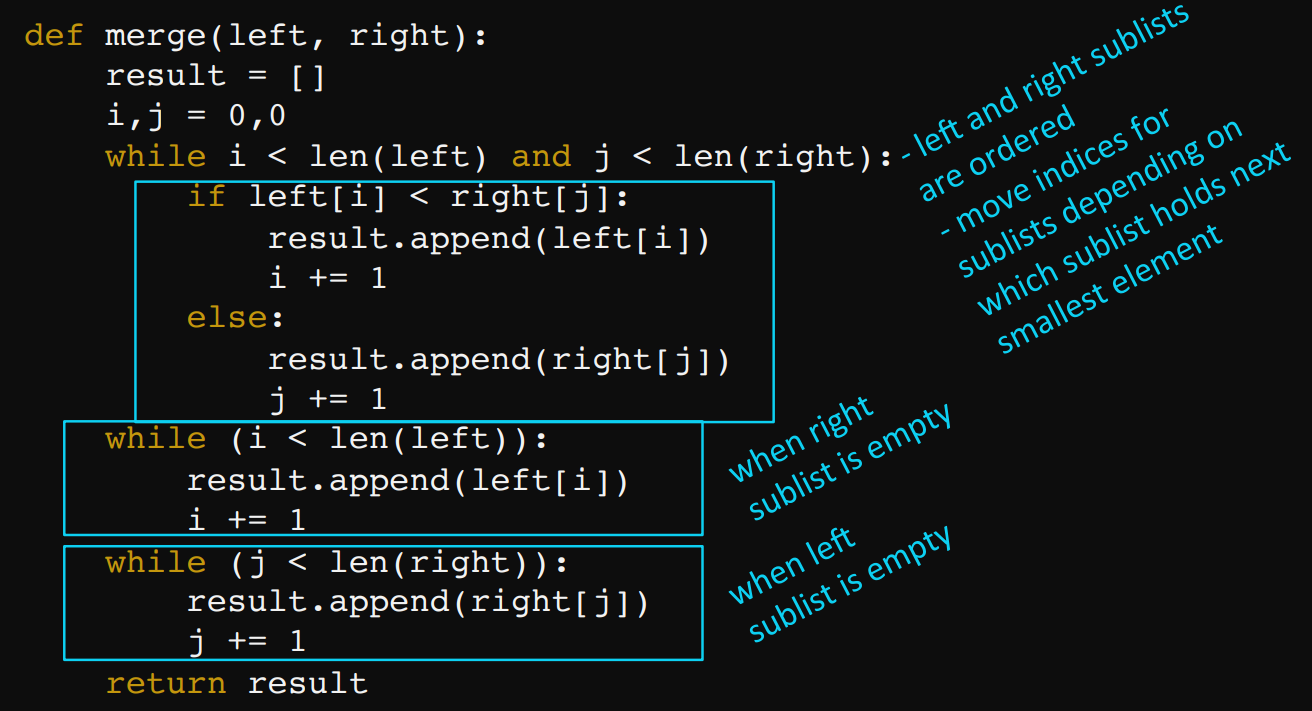
\includegraphics[width=.9\linewidth]{./Screenshot 2022-03-16 100339.png}
\end{center}
\begin{center}
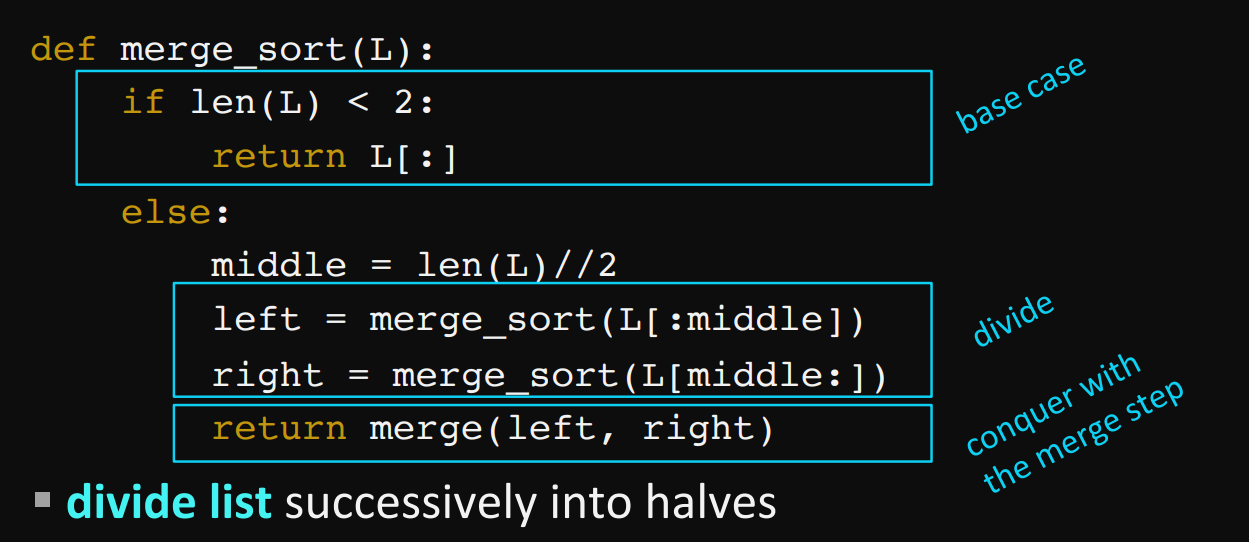
\includegraphics[width=.9\linewidth]{./Screenshot 2022-03-16 100418.png}
\end{center}
\subsection{Changes}
\label{sec:org36b19cc}
\begin{itemize}
\item Variable names were changed for consistency.
\item Assignation of "middle" incorporates int() for readability.
\item "<=" used instead of "<" in "merge" to make sort stable.
\end{itemize}
\section{isSorted}
\label{sec:org8a11782}
Take from Stack Overflow.
Title: Pythonic way to check if a list is sorted or not
\url{https://stackoverflow.com/questions/3755136/pythonic-way-to-check-if-a-list-is-sorted-or-not}
\begin{center}
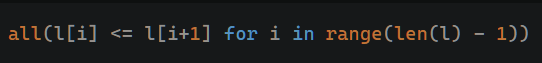
\includegraphics[width=.9\linewidth]{./Screenshot 2022-03-18 083426.png}
\end{center}
\end{document}